\section{Methods} \label{sec:methods}

\subsection{Distance metrics}

The following sections describe a range of different types of distance metrics,
that is, methods for measuring the distance between sequences.

\subsubsection{Edit distance}

One type of \emph{edit distance} is the \emph{Levenshtein
distance}~\cite{levenshtein}, which is a string metric for determining the
similarity between two sequences. It is defined to be the minimum number of
edits to transform the first sequence into the other~\cite[p.~52]{dong}.

The edit operations consists of \emph{insertions}, \emph{deletions} and
\emph{substitutions}. These operations are, respectively, inserting a letter,
removing a letter and changing one letter into another.

For example, the two sequences
\begin{center}
  \texttt{ACGT} \\
  \texttt{ACGGC}
\end{center}
would have a distance of 2 (e.g. substituting T for G and inserting a C). However,
there are some cases where the relevance of the distance is arguable. Consider
the sequences
\begin{center}
  \texttt{AACC} \\
  \texttt{CCAA}
\end{center}
with a distance of 4. The two sequences actually have the maximal distance
possible even though one is just a reversal of the other. Since reversals of
substrings are commonly observed in sequence data~\cite{arslan}, this result
might not be appropriate.

%A naive version of the Levenshtein distance metric was implemented, but as
%expected, this is absolutely useless in any practical setting, since it does
%not reuse already calculated results. Therefore, this was quickly transformed
%into a dynamic programming solution, which solves subproblems just once, stores
%and reuses the intermediate results. This dynamic programming bottom up
%solution was however still very slow, yielding a performance of around 70
%comparisons per second.

A bottom-up dynamic programming version of the Levenshtein distance metric was
implemented and tested on real DNA/RNA data to evaluate its performance, and it
was clear that this algorithm is not suitable for large data sets, because it
would be infeasible to complete even a linear time clustering, in the number of
sequences to be clustered. The implementation could most likely be optimized
further, but because of the characteristics of an edit distance algorithm like
Levenshtein and because of the performance requirements for this project, it
was decided to not pursue further optimization and instead focus on other types
of algorithms. Furthermore, the Levenshtein distance penalizes reversals, i.e.
it results in an increased distance.

The Levenshtein distance can still be used for evaluation and benchmarking
against other metrics. The algorithm is attached in appendix
\ref{app:levenshtein_algorithm} and results from tests are shown in section
\ref{sec:results}.

As stated in \cite[pp.~1-2]{andoni}, ``The worst-case running time known for
this problem has not improved in three decades (..)'', specifically it states
that the running time of Levenshtein is $\mathcal{O}(d^2)$, where $d$ is the
length of the two sequences, and $\mathcal{O}(d^2/\log_2(d))$ for a constant
size alphabet. It further supports the conclusion that the running time of the
Levenshtein algorithm is too poor for the large data sets of the problem
domain.
% TODO: what if their lengths are different?

This lack of improvements of the performance of edit distance is one motivation
for the introduction of the concept of sequence alignment.

%The implemented dynamic programming solution has a running time of $O(nm)$,
%where $n$ and $m$ are the lengths of the sequences, and this running time seems
%to be inherent in this approach to measuring distance between sequences, as it
%needs to consider all possible edits to one sequence for each position in the
%other sequence.


\subsubsection{Sequence alignment}

\emph{Sequence alignment} is used in bioinformatics to identify regions of
similarity by aligning the characters of two or more sequences in a certain
manner. Besides shifting a sequence to a side, gaps can be inserted between
characters as well. A gap is represented with '-' and it indicates an insertion
in one sequence or a deletion from another sequence. This is called an
\emph{indel}, which is a contraction of the first letters from insertion and
deletion. If it is not have an indel and all characters in the column are same,
then it is a match. Otherwise, it is a mismatch~\cite[pp.~135-136]{dong}.

\begin{figure}[H]
  \centering
  \verb+ATGCAACGA+ \\
  \verb+ |||  |||+ \\
  \verb+-TGCG-CGA+
  \caption{Sequence alignment of `ATGCAACGA' and `TGCGCGA'}
  \label{fig:seq_alignment}
\end{figure}

Figure \ref{fig:seq_alignment} displays an alignment of two sequences. In
column 0 is an indel, in columns 1-3 are matches, in column 4 is a mismatch and
so forth. The vertical bar characters in the middle line, indicates matches.

% TODO: describe Needleman-Wunch
%The
%number of each type can then be used in a formula to calculate the similarity
%between the sequences. Note that more than two sequences can be aligned in a
%\emph{multiple sequence alignment}.
%
%There are many alignments and among those are optimal alignments, which are
%strived to be found or . Among those is an optimal alignment which is the one
%that is searched for.

Both \texttt{UCLUST} and the very recent project \texttt{VSEARCH} uses some
kind of sequence alignment for comparing sequences. \texttt{VSEARCH} uses a
parallelized version of the dynamic programming algorithm Needleman-Wunsch,
while \texttt{UCLUST} uses a heuristic procedure by default, but can be
instructed to use full dynamic programming with either the Needleman-Wunsch or
Smith-Waterman algorithm. However, this will make \texttt{UCLUST} much
slower.~\cite{vsearch} The heuristic algorithm used in \texttt{UCLUST} gives an
approximation of the optimal alignment for the purpose of increased
performance, but the alignment is not guaranteed to be optimal.

As opposed to \texttt{USEARCH}, \texttt{VSEARCH} is free and open-source
software and is designed for 64-bit processors, so it does not have the
limitation on usable memory that the free, 32-bit version of \texttt{USEARCH}
has.

Sequence alignment is still a computationally expensive operation and for
comparison of sequences with low similarity, the results of sequence alignment
are often poor. Additionally, as with the Levenshtein distance metric, sequence
alignment is very sensitive to the ordering of parts of sequences.
\emph{Alignment-free} sequence comparison methods strive to provide a measure
of sequence similarity while avoiding the costly computation that alignment
involves. Alignment-free comparison allows one to look at each of the sequences
independently, extracting some characteristics, or \emph{features}, of the each
sequence and then comparing these characteristics.  This can possibly reduce
the complexity of the comparison to linear time or better. One such
alignment-free method, is $k$-mer counting which will be presented and analyzed
in the following section.


\subsubsection{Feature based distance} \label{sec:kmer_distance}

A $k$-mer, or $k$-gram or simply a \emph{word}, is a subsequence of length
$k>0$ over some alphabet $\mathcal{A}$ of a sequence. An interesting feature of
a sequence is which $k$-mers occur in that sequence and how many times they
occur. This is called \emph{$k$-mer counting} and is a type of \emph{feature
based distance metric}.

The \emph{$d2$ distance metric} is a feature based distance metric, using
$k$-mers as the feature. The distance is calculated by counting the $k$-mers
occurring in two sequences, representing these occurrences as two vectors and
finally taking the Euclidean distance between these two
vectors~\cite[pp.~53-54]{dong}.

Let $c_x(w)$ be the number of times that a $k$-mer $w$ occurs in the sequence
$x$. Then the $d2$ distance between two sequences, $x$ and $y$, can be defined
as follows~\cite[pp.~1-2]{hazelhurst}
\begin{equation}
  d2_k(x,y) \eqdef \sqrt{\sum_{w \in K(x) \cup K(y)} (c_x(w) - c_y(w))^2}
\end{equation}
where $K(x)$ and $K(y)$ denotes the set of $k$-mers in $x$ and $y$,
respectively.

As an example, the two $2$-mer frequency vectors of the sequences
\begin{align*}
  S_1 &= ACTACAC \\
  S_2 &= ACAGAT
\end{align*}
over the alphabet $\mathcal{A} = \{A,C,T,G\}$, can be illustrated as follows:

\begin{table}[!h]
\centering
\scalebox{0.75}{
\begin{tabular}{c | c c c c c c c c c c c c c c c c}
        & AA & AC & AG & AT & CA & CC & CG & CT & GA & GC & GG & GT & TA & TC & TG & TT \\
  \hline
  $S_1$ &    &  3 &    &    &  1 &    &    &  1 &    &    &    &    &  1 &    &    &    \\
  \hline
  $S_2$ &    &  1 &  1 &  1 &  1 &    &    &    &  1 &    &    &    &    &    &    &    \\
\end{tabular}}
\end{table}

The Euclidean distance would then be calculated as
\begin{align*}
  d2_2(S_1, S_2)
    &= \sqrt{(3-1)^2 + (-1)^2 + (-1)^2 + (1-1)^2 + 1^2 + (-1)^2 + 1^2} \\
    &= \sqrt{9} = 3
\end{align*}

The first version of the $d2$ distance metric algorithm described above, is
shown in algorithm \ref{alg:d2_basic} and it has been implemented as well. The
substring method extracts up to $k$ characters beginning at index $i$ of the
string. This algorithm maintains a single frequency vector, as a map structure
to allow for large $k$ which results in a large number of possible different
$k$-mers. When iterating through the first sequence, $k$-mer counts are
incremented and when iterating through the second sequence, they are
decremented. Finally all the frequencies are squared and the square root of the
sum is returned, corresponding to the Euclidean distance between frequency
vectors for the two sequences.

\begin{algorithm}
  \caption{Basic \textsc{d2} distance metric}
  \label{alg:d2_basic}
  \begin{algorithmic}[1]
    \Require{$s$ and $t$ are DNA or RNA sequences and $k \in \mathbb{Z}^+$}
    \Statex
    \Function{d2}{$s, t, k$}
      \State initialize \texttt{freq\_map} of type \texttt{string $\to$ int} map
      \For{$i \gets 0$ to $length(s) - k$}
        \State \texttt{freq\_map}[$s$.substring($i$, $k$)]\texttt{++}
      \EndFor
      \For{$i \gets 0$ to $length(t) - k$}
        \State \texttt{freq\_map}[$t$.substring($i$, $k$)]\texttt{--}
      \EndFor
      \State $total \gets 0$
      \ForAll{$e \in$ \texttt{freq\_map}}
        \State $total \gets total + e.value^2$
          \Comment{calculate the Euclidean distance}
      \EndFor
      \State \Return $\sqrt{total}$
    \EndFunction
  \end{algorithmic}
\end{algorithm}

To better support the measurement of distance between two sequences of
different length, but similar substrings, the concept of a \emph{window} can be
introduced. In this context, a window is a conceptual construction which gives
a view of fixed length substrings of two sequences. This window can then be
moved step by step over the two sequences, calculating the distance for each
position of the window and then using the lowest of those distances as the
resulting distance. In this way two sequences, where one is a prefix or postfix
of the other, will have zero distance. This concept is illustrated in figure
\ref{fig:d2_window_concept} where the blue box corresponds to the window, which
in this case has the length 10.

\begin{figure}[H]
\centering
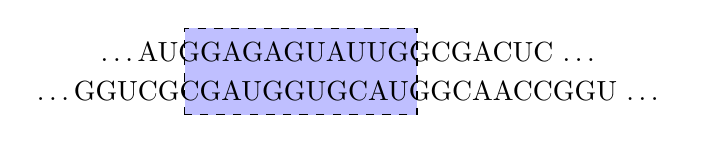
\begin{tikzpicture}
  \draw [fill=blue!25,dashed] (0,0.7) rectangle (2.95,1.8);
  \node at (2.1,1.5) {\dots AUGGAGAGUAUUGGCGACUC \dots};
  \node at (2.1,1.0) {\dots GGUCGCGAUGGUGCAUGGCAACCGGU \dots};
\end{tikzpicture}
\caption{Illustration of the concept of a window.}
\label{fig:d2_window_concept}
\end{figure}

For simplicity, the window size can be set equal to the size of the shortest of
the two sequences. Then the window only moves step by step over the longer of
the two sequences, while maintaining the position, and the $k$-mer counts, for
the shorter sequence.

Figure \ref{fig:d2_window_example} shows an example of this, where the $d2$
distance with the window is 0, since the first sequence is a prefix of the
other, while the $d2$ distance without a window gives a distance of 2.

\begin{figure}[H]
\centering
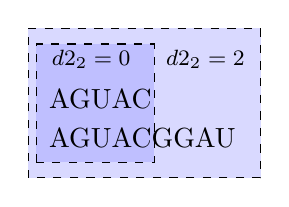
\begin{tikzpicture}
  \draw [fill=blue!15,dashed] (-0.45,0.5) rectangle (2.5,2.4);
  \draw [fill=blue!25,dashed] (-0.35,0.7) rectangle (1.15,2.2);
  \node at (1.0,1.5) {AGUAC\phantom{GGAU}};
  \node at (1.0,1.0) {AGUACGGAU};

  \node at (0.35, 2.0) {\footnotesize $d2_2 = 0$};
  \node at (1.8, 2.0) {\footnotesize $d2_2 = 2$};
\end{tikzpicture}
\caption{Example of difference in distance with window.}
\label{fig:d2_window_example}
\end{figure}

The $d2$ distance metric used in this project uses a window of length equal to
the shortest of the two sequences being compared. The distance between the
substrings in the initial, leftmost position of the window is calculated using
the basic \textsc{d2} algorithm described above.

The window then iterates over the longer sequence and calculates the new
distance between the substring of the longer sequence and the shorter sequence.
This calculation is done using a kind of forward differences method for
reducing the calculations to a few fixed operations for calculating the
distance in the next window from the distance in the current window. This
concept is described in~\cite{hazelhurst}.

% TODO: don't skip straight to Manhattan distance.

Let $|s|$ be the length of the shortest of the two sequences. To begin with
the, the $k$-mers in the first $|s|$ characters of each sequence are counted
and the \emph{Manhattan distance} between these two frequency vectors is
calculated using. The Manhattan distance is similar to the Euclidean distance
but with squaring replaced with absolute value and the square root omitted,
i.e.  for $u, v \in \mathbb{Z}^n$,

\begin{equation}
  d_{Manhattan} \eqdef \sum_{i=1}^{n} |u_i - v_i| \;.
\end{equation}

This distance metric was chosen for simplicity, to make the calculation of
distance in subsequent window positions easier, which also improves
performance, and since there is evidence in the literature that the Manhattan
distance generally is preferable to Euclidean distance for high dimensional
distance calculation~\cite{aggarwal}.

This distance is the distance between the subsequences in the first position of
the window. To calculate the distance in the following window, i.e. advancing
the window through the longer of the two sequences by one character, it is
decided which $k$-mers exit and enter the window, respectively, and then by
looking at whether the existing $k$-mer count in the frequency vector is
negative or positive, it can be decided whether the distance increases or
decreased by 2 or whether it stays the same. Subsequently, the frequency vector
is updated to reflect the change in the new window. The following illustrates
the idea of a window and $k$-mers exiting and entering the window:

%%\node at (4.3,1.5) {AUGGAGAGUAUUGGCGACUC\phantom{ACCGGU \dots}};
%%\node at (4.3,1.0) {GGUCGCGAUGGUGCAUGGCAACCGGU \dots};
%\begin{figure}[H]
%\centering
%\begin{tikzpicture}
%  \draw [fill=blue!25,dashed] (0,0.7) rectangle (3.95,1.8);
%  \node at (4.0,1.5) {ACTGATCGTAGCTAGCTAGTGTTG\phantom{TAGCTAAGCTTAGCTGATCG \dots}};
%  \node at (4.0,1.0) {ACGTAGATCGTGGATGGCTGATCGTAGCTAAGCTTAGCTGATCG \dots};
%\end{tikzpicture}
%\caption{Illustration of the concept of a window.}
%\label{fig:d2_forward_differences}
%\end{figure}

\begin{verbatim}
      |---- window ----------|
      ACTGATCGTAGCTAGCTAGTGTTG
      ACGTAGATCGTGGATGGCTGATCGTAGCTAAGCTTAGCTGATCG.....
      ^^^^                 ^^^^
      k-mer exiting        k-mer entering
\end{verbatim}

The Manhattan distance can be hard to use in practice, because it is very
dependent on the length of the shortest sequence (the length of the window),
the concept of the \emph{Jaccard index}~\cite{jaccard1901,jaccard1912}, or the
\emph{Jaccard similarity coefficient}, is used to ``normalize'' the distance to
a value in the interval $[0,1]$.

The Jaccard index of two sets $A$ and $B$ is defined as follows:
\begin{equation}
  J(A, B) \eqdef \frac{|A \cup B| - |A \cap B|}{|A \cup B|}
\end{equation}
 % TODO:  maybe actually Jaccard distance

In the context of $k$-mer frequencies, the union can be interpreted as the
total number of $k$-mers in the window in the two sequences, and the
intersection as the Manhattan distance in the window.

An algorithm \textsc{K-Dist} for calculating the $d2$ distance, using windows
and the Jaccard index, has been designed and implemented. This is the distance
metric used in the \texttt{klust} program.

\begin{algorithm}
  \caption{\textsc{K-Dist} algorithm}
  \label{alg:K-Dist}
  \begin{algorithmic}[1]
    \Require{$s$ and $t$ are DNA or RNA sequence, $k \in \mathbb{Z}^+$ and $thrs\in [0,1]$ }
    \Statex
    \Function{d2}{$s, t, k, thrs$}
      \State set $s$ to the shortest sequence and $t$ to the longest sequence
      \State initialize array \texttt{kmers} of size $4^k$
      \State $cur\_dist \gets 0$
      \For{$i \gets 0$ to $length(s) - k$}
        \State \texttt{kmers}[$s$.substring($i$, $k$)]\texttt{++}
        \Comment{\parbox[t]{.3\linewidth}{$k$-mer counting}}
        \State \texttt{kmers}[$t$.substring($i$, $k$)]\texttt{-{}-}
      \EndFor
      \ForAll{$c \in$ \texttt{kmers}}
        \State $cur\_dist \gets cur\_dist + |c|$ \Comment{\parbox[t]{.3\linewidth}{Manhattan distance}}
      \EndFor
      \State $min\_dist \gets cur\_dist$
      \For{$i \gets 0$ to $length(t) - length(s)$} \Comment{\parbox[t]{.3\linewidth}{No. of windows}}
        \State \texttt{kmers}[$t$.substring($i$, $k$)]\texttt{-{}-}
        \State \texttt{kmers}[$t$.substring($length(s)-k+i+1$, $k$)]\texttt{++}
        \State update $cur\_dist$ to current Manhattan distance
        \State set $min\_dist=min(min\_dist, cur\_dist)$
      \EndFor
          \State $total \gets 2(length(s)-k+1)$ \Comment{\parbox[t]{.3\linewidth}{Maximal distance}}
      \State \Return{$(total-min\_dist) / total$} \Comment{\parbox[t]{.3\linewidth}{Jaccard index}}
    \EndFunction
  \end{algorithmic}
\end{algorithm}


\subsection{Cluster analysis algorithms}

There are several approaches to clustering sequence data. This section describes different clustering paradigms. It discusses strength, weaknesses and potential in the methods.

\subsubsection{Hierarchical clustering}

%TODO: Add divisive or explain why not.
There are typically two types of hierarchical clustering algorithms, the
agglomerative type that works in a bottom-up manner and the divisive type that
has a top-down approach. This section describes the agglomerative version. In
the agglomerative version all sequences start as leaves in a tree, where the
leaves are considered clusters. Each cluster is then merged together with the
closest cluster, thus building a tree, level for level, until there is only one
cluster left. This gives a hierarchy of the clusters. Alternatively, when the
clustering is based on a similarity threshold, as in this project, the clusters
are merged until no more clusters can be merged. The algorithm is visualized in
figure \ref{fig:hierarchical_clustering}.

\begin{figure}[h!]
  \centering
  \def\svgwidth{\columnwidth}
  \import{graphics/}{Hierarchical_Clustering.pdf_tex}
  \caption{Illustration of agglomerative hierarchical clustering. Clusters,
    with objects represented as letters, are merged with nearby clusters based
    on lexicographic order until there is only one cluster.}
  \label{fig:hierarchical_clustering}
\end{figure}

This addresses the question of what is required for a cluster to be "close" to
another. Besides measuring similarity between sequences with some distance
metric, a definition for when clusters should be merged is needed. The
following is described with respect to that merges happen based on a similarity
threshold.

In the \textit{complete-linkage} approach, all sequences from one cluster must
be above the threshold of all sequences from the other. In the
\textit{average-linkage}, the average distance of all sequence pairs is
required to be above the threshold. With the \textit{single-linkage} approach,
only a sequence from both clusters need an identity above the similarity
threshold.

The complete-linkage approach is computationally very heavy as each merge will
take $\mathcal{O}(mn)$ time, where $m$ and $n$ are the sizes of the clusters.
The average-linkage method is equally computationally hard. This is not viable
for a quick clustering algorithm.

However, the single-linkage approach is often used in sequence
clustering~\cite[pp. 62-63]{dong}. It has the advantage of behaving greedily
and stopping early if a link meets the similarity criterion instead of
calculating all links to find the minimal distance. Though the greedy behavior
can boost performance, it could make a very rough clustering as two sequences
from the clusters might be very similar while other sequences could have a very
low similarity to each other.

There exists an agglomerative method using single-linkage with complexity
$\mathcal{O}(n^2)$ known as SLINK~\cite{sibson} and another using complete-
linkage~\cite{defays}. As the naive agglomerative method, both algorithms build
a distance matrix and then uses row and column elimination but is optimized to
$\mathcal{O}(n^2)$ instead of $\mathcal{O}(n^3)$. Even though $\mathcal{O}(n^2)$
is too heavy for the scope of this project, it produces optimal results and
builds the entire hierarchy. With a greedy single-linkage approach and without
building the entire hierarchy, the complexity could be significantly reduced.
The distance matrix itself takes $n^2$ time to create, which is already too
much, so this indicates the computation of the distances and therefore the
merges should be an ongoing process with the clustering.

\subsubsection{Graph based clustering}

The general framework of graph-based clustering consists of two steps. First
step is to generate a weighted graph from the sequences. The second step, the
clustering step, is to split the graph into subgraphs, which correspond to the
clusters~\cite[pp. 64-65]{dong}.

Consider a graph $G$ with a set of vertices $V$ and a set of edges $E$. In
graph based clustering, we consider $V$ as the set of sequences and $E$ is the
set of similarity scores. The first step is to calculate all $E_{ij}$, the
similarity score between $V_i$ and $V_j$, based on some distance metric. If the
clustering is based on a similarity threshold, edges that are below the
similarity threshold can be ignored.

There are many variants to the clustering step. The reference~\cite{hartuv}
presents an algorithm that tries to minimize edges that connect two subgraphsb by
moving vertices from one subgraph to another.

The reference~\cite{kawaji} tries to maximize the density of edges in a
subgraph. This is done by converting the tree into a simpler tree by removing
all edges that are under the similarity threshold.

Since both of these requires that all edges' weights has been computed, it is
already too slow for efficient sequence clustering. If the subgraphs could be
constructed while computing distances, the time complexity could be reduced.
Both hierarchical and graph based clustering indicates that a heuristic
clustering is needed to obtain the desired performance.

\subsubsection{Greedy algorithm like \texttt{UCLUST}}
The \texttt{UCLUST} algorithm is greedy and is developed so that all member
sequences have similarity $\geq$ $T$ to their centroid.  It works by processing
one sequence at a time and comparing these to the existing centroids. If a
match is found, the sequence is assigned to the matching centroid, otherwise it
becomes a centroid of a new cluster.

It is designed to also support that each centroid has a similarity $<T$ to all
other centroids, but this is not guaranteed to hold. The reason is that the
algorithm only compares a sequence to a prespecified number of centroids given
by the \texttt{-maxrejects} parameter.

It uses the $k$-mer counts to locate centroid candidates for a match, though
how it does it is not very well described.

The similarity calculations are performed with global sequence alignments as
\cite{usearch_algorithm} claims that using the word counts to calculate
identity is not sensitive enough. Greedy clustering is illustrated in figure
\ref{fig:greedy_clustering}.

\begin{figure}[h!]
  \def\svgwidth{\columnwidth}
  \import{graphics/}{Greedy_Clustering.pdf_tex}
  \caption{Illustration of greedy clustering. Sequences are processed in the order they are read. They either become a centroid for a new cluster or they are assigned to an existing cluster.}
  \label{fig:greedy_clustering}
\end{figure}


%TODO? \subsubsection{Greedy algorithm with recalculation of centroids}

% Background: theoretical overview of the field of clustering

\subsection{Naive, greedy clustering algorithm}

A very simple, naive, greedy clustering algorithm, \textsc{Naive\_Clust}, has
been implemented and will be described briefly in this section.

Given a list of sequences and an initially empty list of centroids, the
algorithm works by iterating through the sequences and for every sequence, it
iterates through the list of centroids until a match is found or until the end
of the list. If a match is found, the sequences is added to the cluster
represented by the matching centroid, and otherwise the sequences becomes a new
centroid and is appended to the end of the list of centroids.

% TODO: complexity of algorithm
% This running time of this algorithm depends on the number of clusters in the
% output and therefore it might be around $O(c^2)$, where $c$ denoted the
% number of sequences, in the worst case where the number of clusters is equal
% to the number of sequences.  %O(k*(k-1)/2)

% TODO: refer to algorithm and implementation

This approach is not very useful in practice since it is very computationally
expensive in the worst case. The running time of the algorithm is very dependent
on the ordering of the sequences since the centroids will be in the same order
as in the list of sequences (i.e. the list of centroids is a subsequence of the
list of sequences) and if the first number of sequences happens to be good
centroids, which will match a lot of sequences, the algorithm will perform good
since the search for a centroid will end very early. However, if the first
sequences happen to be very dissimilar from the rest of the data, then these
will become centroids and will be compared against on every iteration even
though they might potentially never match anything.

Thus, there is a motivation to try and create more structure in the collection
of centroids, improve the search for a centroid to compare with the query
sequence or improving the ordering of the centroids.

% The problem with this approach is that it is potentially very computationally
% expensive to possible traverse the entire list of centroids for each
% iteration

% TODO: maybe mention the reason for introducing max_rejects and clustering
% algorithm based on greediness


\subsection{\textsc{Simple\_Clust} algorithm}

Another clustering algorithm, named \textsc{Simple\_Clust}, was developed and
implemented, and will be described in this section. \textsc{Simple\_Clust}
tries to address some of the problems with the \textsc{Naive\_Clust} algorithm
by imposing more structure on the collection of centroids and by giving up
after some fixed number of comparisons of a given query sequence.

\textsc{Simple\_Clust} works by iterating sequentially through the sequences to
be clustered; the $max\_reject$ most frequent $k$-mers for the query sequence
are calculated and for each of these most frequent $k$-mers, a centroid which
has that $k$-mer as the most frequently occurring one (if one such centroid
exists) is compared with the query sequence to check if their similarity is
above the given threshold. The query sequence is assigned to the cluster for the
first centroid that matches the query sequence; if no such centroid is found,
out of the maximum possible $max\_reject$ number of tries, the query sequence
becomes a centroid for a new cluster and is added to the collection of centroids
along with the information about the most frequently occurring $k$-mer in the
sequence. Pseudocode for the algorithm is attached in appendix \ref{app:simple_clust}.


\begin{algorithm}
  \caption{\textsc{Simple\_Clust}}
  \label{alg:simple_clust}
  \begin{algorithmic}[1]
    \Require{$S$ is an array of [DR]NA sequences, $k \in \mathbb{Z}^+$ and
             $max\_rejects \in \mathbb{Z}^+$, $id \in [0,1]$}
    \Statex
    \Function{Simple\_Clust}{$S, k, max\_rejects$}
      \State $cluster\_count \gets 0$
      \State $centroids \gets []$ \Comment{map from $k$-mer to sequence}
      \ForAll{$s \in S$}
        \State $mfk \gets$ $max\_rejects$ most frequent $k$-mers in $s$
        \ForAll{$m \in mfk$}
          \If{$centroids[m]$ does not exists}
            \State continue
          \ElsIf{$distance(s, centroids[m]) \geq id$}
            \State add $s$ to cluster with centroid $centroids[m]$
            \State break
          \EndIf
        \EndFor
        \If{matching centroid was not found}
          \State centroids.insert(mfk[0], s)
        \EndIf
      \EndFor
      \State \Return $cluster\_count$
    \EndFunction
  \end{algorithmic}
\end{algorithm}

>>>>>>> ff45d07e36dd25b5fc11d9db1c815c5608b7542c

This algorithm did not perform as well as hoped, in particular for larger $k$
the number of different possible $k$-mers increases exponentially and for e.g.
$k = 6$ and a four letter alphabet, there are $4^6 = 4096$ different $k$-mers
and therefore the lookup in line 7 of the algorithm will often be unsuccessful.
Additionally, the most frequently occurring $k$-mer did not appear to be a
sufficiently good characteristic for choosing a centroid that is likely to
match, as it is seen from the evaluation in section \ref{sec:results}. To
clarify, the correspondence between the most frequently occurring $k$-mer of
two sequences and the similarity of the sequences, is evidently not very strong.
% TODO


\subsection{\textsc{Prioritized\_Intersect\_Clust}}

This section describes another clustering algorithm that was developed and
implemented, named \textsc{Prioritized\_Intersect\_Clust}, which looks at the
set of $k$-mers occurring in the query and target sequences and bases the
decision of whether to try comparing or not, on the cardinality of the
intersection between these sets. This way, the search for a likely match is not
just determined by the single most frequently occurring $k$-mer, as with
\textsc{Simple\_Clust}, but rather all the occurring $k$-mers, regardless of
their count. Additionally, the centroids are stored in a doubly linked list and
whenever a centroid matches a sequence, that centroid is moved to the front of
the list. This makes the algorithm less sensitive to the ordering of the input
sequences. The choice of the centroids will still be made greedily though, in
lack of well-performing alternatives, but the algorithm should nonetheless be
less prone to bad performance caused by an unlucky ordering of the input
sequences. Algorithm \ref{alg:intersect_clust} shows pseudocode for the
\textsc{Prioritized\_Intersect\_Clust} algorithm.

%TODO: Move some of it to results? SILVA not introduced.
The idea of moving a matching centroid to the front of the list is, among other
things, inspired by the observation that the results from \texttt{UCLUST} and
\texttt{VSEARCH} often contain a large number of very small clusters and even
singleton clusters, i.e. clusters consisting of just a single sequence. For
example, clustering the data set \texttt{SILVA\_119\_SSURef\_tax\_silva.fasta}
with \texttt{USEARCH} and a similarity threshold of $0.95$, gives 117,205
clusters out of which 67,410 clusters are singleton clusters, that is more than
half of the clusters. These results are shown in figure \ref{fig:uclust_silva}
in section \ref{sec:results}.

\begin{algorithm}[H]
  \caption{\textsc{Prioritized\_Intersect\_Clust}}
  \label{alg:intersect_clust}
  \begin{algorithmic}[1]
    \Require{$S$ is an array of [DR]NA sequences, $k \in \mathbb{Z}^+$,
            $max\_rejects \in \mathbb{Z}^+$ and $id \in [0,1]$}
    \Statex
    \Function{Prioritized\_Intersect\_Clust}{$S, k, max\_rejects$}
      \State $centroids \gets [~]$ \Comment{initialize empty list of centroids}
      \ForAll{$s \in S$}
        \State $match \gets false$
        \State $rejects \gets 0$
        \State $close\_match \gets \mathtt{NULL}$

        \ForAll{$c \in centroids$}
          \If{$rejects$ \texttt{==} $max\_rejects$}
            \State $break$
          \EndIf

          \State\Comment{$K(s)$: set of $k$-mers in $s$}
          \If{$|K(s) \cap K(c)| \geq |K(c)| \cdot id$}
            \If{\Call{d2}{s, c, k} $ \geq id$}
              \State Add $s$ to cluster represented by $c$.
              \State Move $c$ to the front of $centroids$.
              \State $match \gets true$
              \State $break$
            \EndIf
            \State
            \If{\Call{has\_link}{c} \texttt{AND} \Call{d2}{s, c.link, k} $ \geq id$}
              \State Add $s$ to cluster represented by $c.link$.
              \State Move $c.link$ to the front of $centroids$.
              \State $match \gets true$
              \State $break$
            \EndIf
            \State $rejects \gets rejects + 1$
            \State $close\_match \gets c$
          \EndIf
        \EndFor
        \State
        \If{$\mathtt{NOT}\ match$}  \Comment{add new centroid to list}
          \If{$close\_match$ \texttt{!= NULL}}
            \State $s.link \gets close\_match$
          \EndIf
          \State Prepend $s$ to $centroids$.
        \EndIf
      \EndFor
    \EndFunction
  \end{algorithmic}
\end{algorithm}
